\documentclass[a4paper,12pt,twocolumn]{article}

\usepackage[papersize={216mm,330mm},tmargin=15mm,bmargin=15mm,lmargin=15mm,rmargin=15mm]{geometry}
\usepackage[english]{babel}
\usepackage[utf8]{inputenc}
\usepackage{amsmath,amssymb}% for \eqref
\usepackage{graphicx}
\usepackage[colorinlistoftodos]{todonotes}
\pagestyle{myheadings}
\markright{Balanced Scorecard y Business Model Canvas}

\title{Balanced Scorecard y Business Model Canvas}
\date{\today}
\begin{document}
\maketitle
\subsubsection*{Abstract}
The Balanced Scorecard (CMI Spanish Acronym) and the Canvas model can be linked as complementary tools for entrepreneurs. The first develops goals and operational measures in four main perspectives for the purpose of achieving the mission and strategy. The second suggest a (re-) evolution in generating business models, establishing nine sections that reflect their logic. In the article a working model is developed that, based on the need for a CMI it relates its design to the information previously collected in the Canvas model, pointing their mutual necessity.
\subsubsection*{Resumén}
El Cuadro de Mando Integral (BSC) y el modelo Canvas pueden enlazarse como herramientas complementarias para los emprendedores. La primera desarrolla objetivos y medidas operativas en cuatro perspectivas principales para alcanzar la misión y estrategia. La segunda ha supuesto una (re-)evolución en la generación de modelos de negocio, estableciendo nueve apartados que reflejan su lógica. En el artículo se desarrolla un modelo de trabajo que, partiendo de la necesidad de disponer de un BSC, relaciona su diseño con la información recogida previamente en el modelo Canvas, señalando su mutua necesidad.

\section{Introducción}
\item{De acuerdo con el informe Global Entrepreneurship Monitor (GEM) del año 2012, a pesar de que en España la actividad emprendedora ha aumentado en los últimos años, son necesarios más esfuerzos para consolidar las nuevas empresas. Se reconoce ampliamente que su desarrollo y supervivencia no depende tanto de tener una buena idea de negocio sino de su adecuada ejecución y gestión. En este sentido, desde diferentes ámbitos se defiende que los emprendedores/as necesitan herramientas que les permitan desarrollar sus estrategias y les indiquen el grado de consecución de sus objetivos y actividades como medio de incrementar su probabilidad de supervivencia (\footnote{Davila & Oyon, 2009}).}

\item{En la literatura de dirección estratégica, el cuadro de mando integral (Balanced Scorecard, BSC de aquí en adelante) se considera como una de las herramientas más conocidas e importantes para la implementación de la estrategia (\footnote{Grant, 2006}). Su utilidad destaca en el momento de desarrollar objetivos operativos para la comunicación de la misión y estrategia de la empresa, así como en la medición del grado de consecución de éstas, proponiendo convertir la estrategia en un conjunto de medidas de actuación que permiten su traducción y gestión (\footnote{Kaplan y Norton, 1992}). De esta forma, un BSC ha de estar constituido por un conjunto limitado de medidas financieras y no financieras organizadas en cuatro principales perspectivas interrelacionadas entre sí (\footnote{Da Silva et al., 2013}), que describen la estrategia organizativa a través de relaciones causa-efecto entre los indicadores: (1) financiera, (2) cliente, (3) interna e (4) innovación y crecimiento.}

\section{OBJETIVOS} 
\\
\textbf{}
\\

\section{MARCO TEÓRICO}
\textbf{2.1 DATA STORYTELLYNG}
\item{El Balanced Scorecard, denominado BSC, es un marco para implementar y administrar la estrategia. Vincula una visión a objetivos estratégicos, medidas, metas e iniciativas. Equilibra las medidas financieras con las medidas de desempeño y los objetivos relacionados con todas las demás partes de la organización. Es una herramienta de gestión del rendimiento empresarial.}

\begin{figure}[h!]
\centering
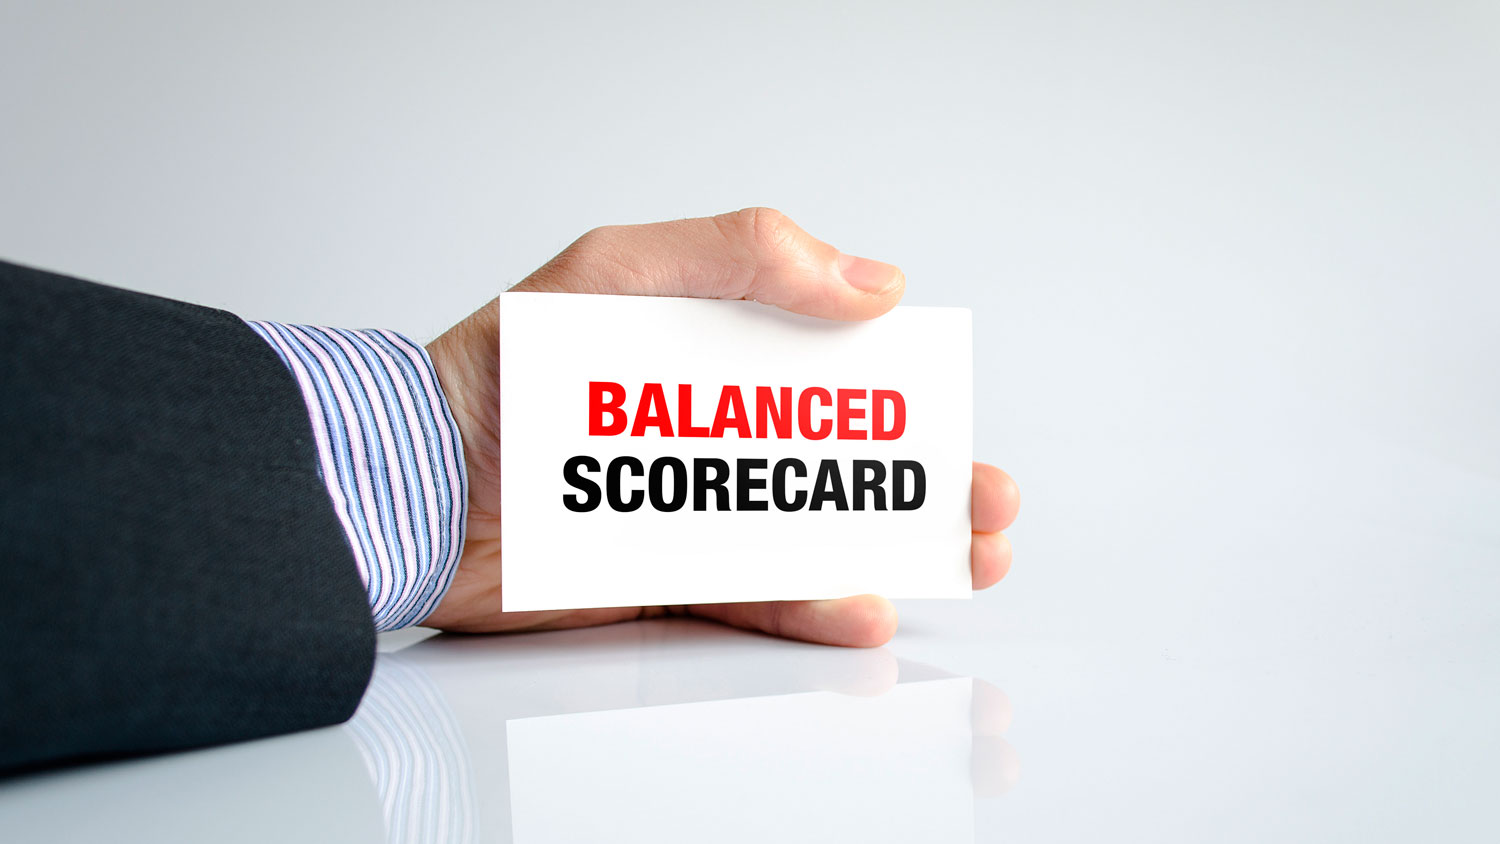
\includegraphics[width=9cm]{./Imagenes/img3}
\end{figure}


\section*{Las cuatro perspectivas}
\item{A menudo surgen preguntas sobre las cuatro Perspectivas descritas en la metodología. ¿Por qué deberíamos considerar solo la capacidad financiera, de clientes, de procesos comerciales y organizativa? ¿Por qué no incluir salud y seguridad? La respuesta es, por supuesto, que nada nos detiene. Las cuatro perspectivas son simplemente un marco. Sin embargo, durante décadas de uso, ha quedado claro que funcionan.

\\
\textbf{}
\\
Más importante aún, existe una relación causal entre las perspectivas. Trabajando de abajo hacia arriba: los cambios en la capacidad organizativa generarán cambios en los procesos comerciales que afectarán a los clientes y mejorarán los resultados financieros. La relación causal puede no estar garantizada si se agrega una nueva perspectiva. El resultado podría ser un cuadro de mando útil, pero no sería, por definición, un cuadro de mando equilibrado.}
\\
\item{En resumen, las cuatro perspectivas del cuadro de mando son:}
\textbf{}

\begin{figure}[h!]
\centering
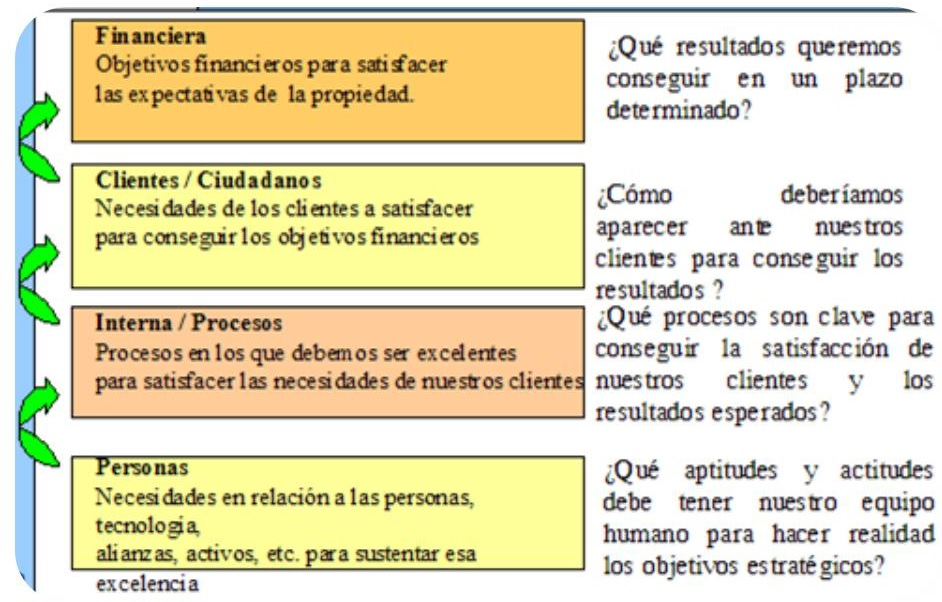
\includegraphics[width=8cm]{./Imagenes/img13}
\caption{\label{fig:01}las cuatro perspectivas}
\end{figure}

\begin{figure}[h!]
\centering
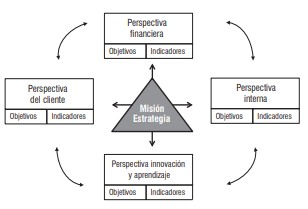
\includegraphics[width=8cm]{./Imagenes/img2}
\caption{\label{fig:01}Misión Estratégica}
\end{figure}

\\
\textbf{}
\\
\\
\begin{figure}[h!]
\centering
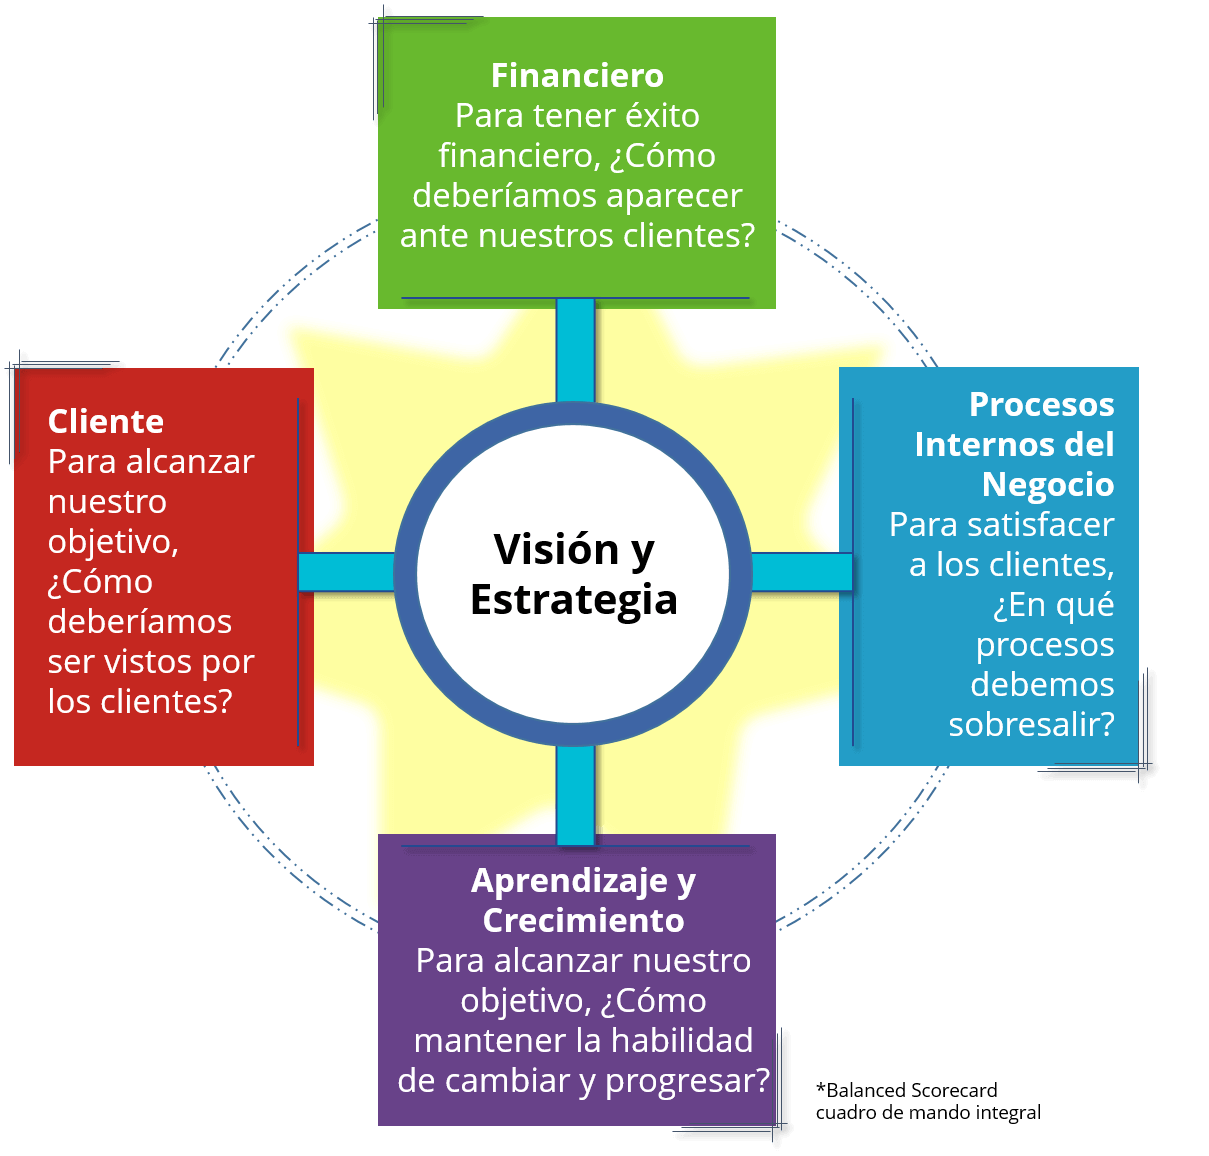
\includegraphics[width=9cm]{./Imagenes/img4}
\caption{\label{fig:01}Visión y Estrategia}
\end{figure}

\section{EJEMPLOS}
\\
\textbf{}
\\

\section{ANÁLISIS (Apreciaciones)}

\\
\textbf{}
\\

\section{CONCLUSIONES} 
\item Como ves, no necesitas ser un “nerd” obsesionado con los datos para entenderlos y para poner bajo los reflectores el valor de los productos o servicios de tu marca. Para eso estamos nosotros: nuestra tarea es hacer las preguntas correctas, entender los puntos más importantes que aporten significado a los hallazgos y ponerlos en contexto, porque lanzar hechos y cifras aleatorios o liberar tablas de Excel con cientos de filas no funciona. 

\item Usar la data con efectividad requiere ser selectivo y aterrizar información en el contexto de la narrativa que estás comunicando para amplificar la conversación sobre tu marca que está teniendo lugar en los medios. Todos estos datos tienen que contar una historia, si no no tienen chiste. Acércate a nosotros para aprovechar toda la información con la que cuentas para generar historias de impacto. Tenemos muchas ideas que compartir contigo  


\subsection*{Sitios Web Relacionados}
\begin{enumerate}
\item Anzola, P., Bayona, C. & García, T. (2015). "La generación de valor a partir de innovaciones organizativas: efectos directos y moderadores". Universia Business Review, 46: 70-93. 
\item Bastidas, E., Ripoll, V. & Moreno, Z. (2011). "Cuadro de mando multidimensional: propuesta de diseño para la empresa pública de transporte ferroviario de mercancías Renfe-operadora-España". Revista Científica Teorías, Enfoques y Aplicaciones en las Ciencias Sociales, 4(8): 65-78.  
\item Da Silva, J., Pastor, A. & Pastor, J. (2013). "El uso del Cuadro de Mando Integral como instrumento de medición para comparar los modelos de excelencia en gestión". Revista Ibero-Americana de Estratégia, 13(4): 18-3
\item Davila, A. & Oyon, D. (2009). "Introduction to the Special Section on Accounting, Innovation and Entrepreneurship". European Accounting Review, 18(2): 277-280. 
\item https://estrategiaspg.wordpress.com/2015/04/-30/el-balanced-scorecard-bsc-parte-1-las-perspectivas/



\item https://www.isotools.org/2015/02/23/que-es-el-balanced-scorecard-conoce-su-funcionamiento-y-ventajas/\\
\item https://economipedia.com/definiciones/modelo-canvas.html\\
\item https://innokabi.com/canvas-de-modelo-de-negocio/\\
\item https://josefacchin.com/modelo-canvas-de-negocio/\\
\item https://www.adaptiveus.com/balanced-scorecard-vs-business-model-canvas/\\
\end{enumerate}


\end{document}